\section{Compartilhando seu código pelo GitHub}

\begin{slide}[method=direct]{Git \& GitHub ?}
	\begin{itemize}
		\item{Git e GitHub são a mesma coisa?}
		\begin{itemize}
		\item{\textit{Não. Git é o sistema de controle de versões, com o qual interagimos na linha de comando. Já o GitHub é uma 					rede social para programadores que disponibiliza repositórios Git acessíveis remotamente.}}
		\end{itemize}
	\end{itemize}

	\begin{center}
	
\includegraphics[width=0.4\textwidth,natwidth=800,natheight=600]{./imagens/Octocat.png}
	\end{center}
\end{slide}

\begin{slide}[method=direct]{Criando um repositório}
	\begin{center}
	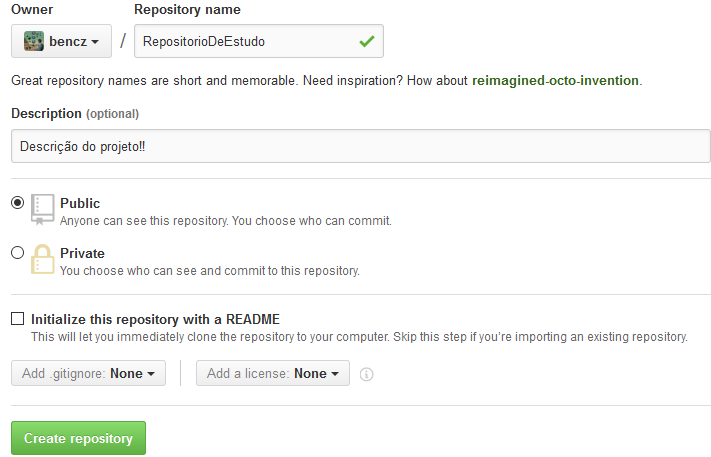
\includegraphics[width=0.9\textwidth,natwidth=711,natheight=457]{./imagens/criando_repo.png}
	\end{center}
\end{slide}

\begin{slide}[method=direct]{Apontando seu projeto para o Git}
	\begin{itemize}
	\item{Agora que já temos um repositório criado no GitHub, temos que apontar o nosso repositorio criado na nossa maquina para o repositório que foi criado no GitHub. \\
	Para isso, use o terminal e navegue até o diretorio onde está o repositorio que nós criamos e então execute a seguinte linha de comando:	}
	\end{itemize}
	
	\begin{lstlisting}[style=Bash,basicstyle=\tiny]
$ git remote add origin https://github.com/bencz/RepositorioDeEstudo.git
          \end{lstlisting}
\end{slide}

\begin{slide}[method=direct]{Enviando para o GitHub}
	\begin{itemize}
	\item{Agora que estamos com o repositório remoto configurado, podemos enviar as mudanças que fizemos para o GitHub.\\
	         Para isso, é necessario executar o comando seguinte comando:
	         \begin{lstlisting}[style=Bash]
$ git push origin master
	         \end{lstlisting}
	         Com este comando enviamos as alterações para o repositório remoto configurado com o nome \textit{origin}. \\
	         O output do comando vai ser algo semelhante com:
	         \begin{lstlisting}[style=Bash,basicstyle=\tiny]
Counting objects: 6, done.
Delta compression using up to 2 threads.
Compressing objects: 100% (3/3), done.
Writing objects: 100% (6/6), 519 bytes | 0 bytes/s, done.
Total 6 (delta 0), reused 0 (delta 0)
To https://github.com/bencz/RepositorioDeEstudo.git
 * [new branch]      master -> master
	         \end{lstlisting}
	         }
	\end{itemize}
\end{slide}

\begin{slide}[method=direct]{Clonando projetos do GitHub}
	\begin{itemize}
	\item{Para clonar um projeto do GitHub, basta utilizar o seguinte comando:
	\begin{lstlisting}[style=Bash]
$ git clone <link do projeto>.git
	\end{lstlisting}
	Quando executado o comando de clone deverá aparecer algo como:
	\begin{lstlisting}[style=Bash,basicstyle=\tiny]
$ git clone https://github.com/bencz/Beryl.git
Cloning into 'Beryl'...
remote: Counting objects: 371, done.
remote: Total 371 (delta 0), reused 0 (delta 0), pack-reused 371
Receiving objects: 100% (371/371), 69.02 KiB | 122.00 KiB/s, done.
Resolving deltas: 100% (248/248), done.
Checking connectivity... done.
	\end{lstlisting}
	}
	\end{itemize}
\end{slide}